Un grupo de 64 obreros puede terminar una obra en 15 días. Al cabo de 5 días de trabajo, se les unen obreros de otro grupo, de modo que tardan 5 días menos en terminar la obra.
\textbf{¿Cuántos obreros había en el segundo grupo?}

\begin{solutionbox}{9cm}
    Sabemos que 64 obreros terminarían la obra en 15 días. Como luego de los primeros 5 días de trabajo llegaron más obreros, hacemos el siguiente gráfico para representar la situación:

    \begin{minipage}{.35\textwidth}
        \begin{figure}[H]
            \centering
            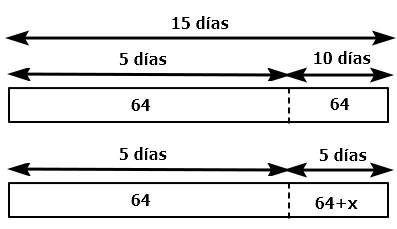
\includegraphics[width=\linewidth]{../images/tableS8L103}
        \end{figure}
    \end{minipage}\hfill
    \begin{minipage}{.55\textwidth}
        Observamos que, en esta situación, a mayor cantidad de obreros, menos días se necesitarán para terminar la obra.
        \begin{table}[H]
            \centering
            \begin{tabular}{|l|c|l|}
                \hline
                Cantidad de obreros         & 64 & 64+x \\
                \hline
                Cantidad de días de trabajo & 10 & 5    \\
                \hline
            \end{tabular}
        \end{table}
        Como es una relación inversamente proporcional, planteamos la siguiente relación:
        \begin{align*}
            64 \times 10 & = 5 \times (64+x) \\
            640          & = 320 +5x         \\
            5x           & = 320             \\
            x            & = 64
        \end{align*}
    \end{minipage}

    En el segundo grupo, había 64 obreros más, es decir, un total de 128 obreros.
\end{solutionbox}